% !TEX root = ./thesis.tex

\chapter{Model}\label{ch:mode}

In this chapter we propose a method for learning a dense manifold from image sequences.
First we provide details about our model initialization and training procedure.
We describe several backbone architectures that can be used a model base.
At last, we describe our method of robust manifold learning.


\section{Training process}

In our training we use a server with Intel Xeon CPU 2.40GHz, 64GB of RAM and a GeForce GTX TITAN X Kepler graphics card with 12GB of video memory. Server runs Debian 8.7 operation system with CUDA 8.0, CuDNN 5.1 and TensorFlow 1.0 installed.

\subsection{Tensorflow}

In deep learning TensorFlow \cite{GoogleResearch2015, Abadi2016}, Torch \cite{torch}, and Caffe \cite{jia2014caffe} are among the most common choices of scientific computing framework.
These frameworks use different underlying programming languages and show different compatibility features and qualities of managing computational resources.

We use TensorFlow as our scientific computing framework of choice.

TensorFlow is an open source cross platform software library.
TensorFlow constructs complex computational procedures in form of computational graphs.
Each node of the graph represents a mathematical operation.
Edges of the graph represent data flows between operations in form of multidimensional arrays, also called \textit{tensors}.
An example of a computational graph of the single-layer perceptron is shown on figure \ref{fig:tf_graph}.

\begin{figure}[h!]
  \centering
    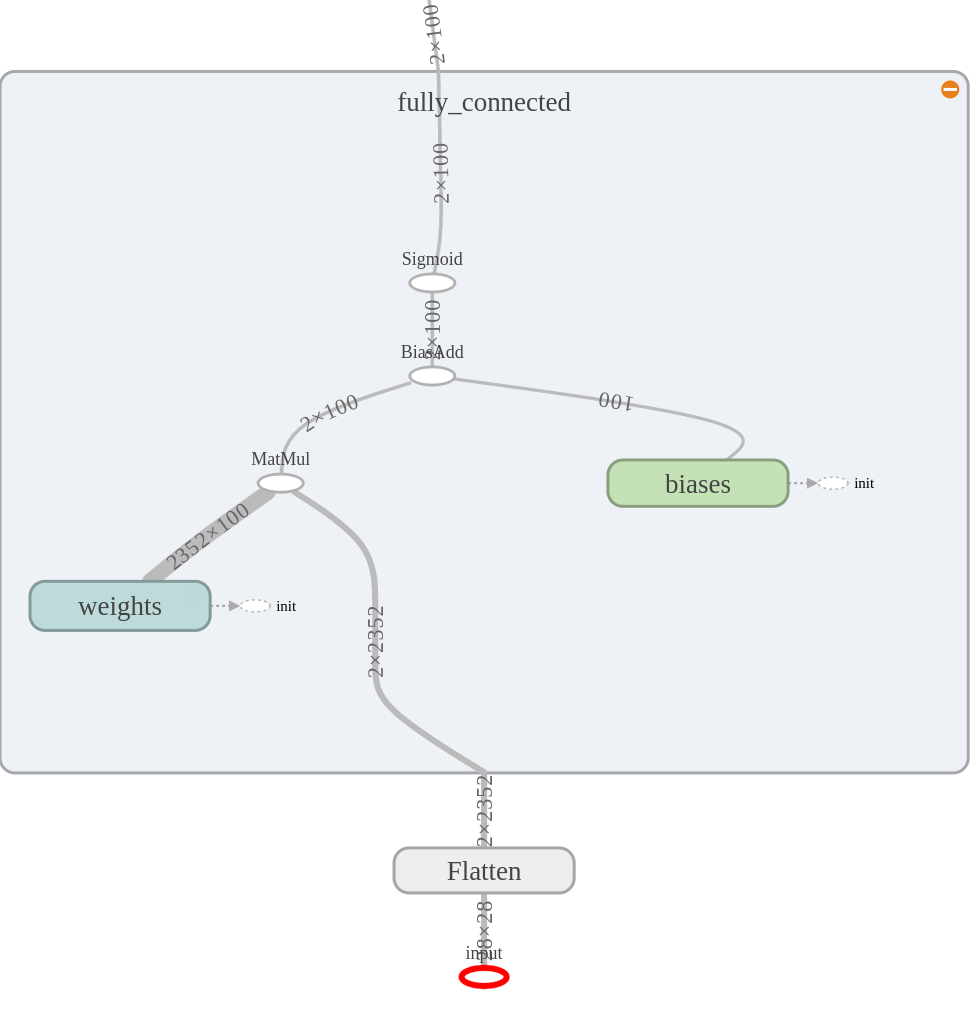
\includegraphics[width=0.7\textwidth,height=0.7\textheight,keepaspectratio]{tf_graph_1.png}
  \caption{TensorFlow detailed graph representation of a single fully connected layer with 100 neurons and sigmoid activation function. Image produced with the TensorBoard visualization tool.}
  \label{fig:tf_graph}
\end{figure}

TensorFlow provides cross platform compatibility, which allows to run code on different types of devices and operation systems.
Abstraction over underlying system allows to run models, build with TensorFlow, both on GPUs and CPU without code changes.
Integration with hight performance computing libraries as CUDA \cite{Nickolls2008} and native support of distributed computing makes it a good candidate for computer vision tasks.
An competition winning family of convolutional neural networks Inception is solely developed and maintained on that platform \cite{Szegedy2016}.

We use TensorFlow as our framework of choice for several reasons.
First of all, being a cross-platform frameworks it enables larger audience to reuse results of our research.
Second, it allows to easily configure and run deep network architecture and, at the same time, apply non-trivial modification to the computational flow.
And, at last, it provides build-in visualization tools that allow better control of the learning process.

All our code is shared for public use under MIT License.
\footnote{\url{https://github.com/yselivonchyk/TensorFlow_DCIGN}}

\subsection{Training algorithm}

We run the training using stochastic gradient descent algorithm with mini-batches.
We use adaptive learning rate in form of Adam update rule.
Adaptive learning rate rule lead to more stable convergence of our models.
These techniques are described in details in chapter \ref{ch:tede}.

We use mini-batch size of 128 as the largest one that fits into video memory.
By grid search, we selected learning rate $n=0.0001$ for all models. This learning rate falls into the interval of recommended learning rates for Adam update rule \cite{Kingma2015}.

As a termination condition of gradient descent algorithm we early stopping \ref{alg:bp}.

Model hyper-parameters, such as learning rate, layers sizes, regularization values and parameters of composite loss function $L=L_{reco} + \alpha L_2 + \beta L_3$ are selected using in a greedy manner.
That is, for a given set of parameters we perform grid search, adjusting a single parameter.
After the search, the best value of the parameter is selected and updated in the parameter set.
Grid search for the next parameter is performed independently while using updated set.
Whenever a single hyper-parameter does not have significant effect on the general performance of the model, the value requiring lower computational complexity is selected.

\subsection{Model weights initialization}

Initial model parameters $\theta$ in conjunction with the learning algorithm play a crucial role in finding a good local minima of the optimization problem.
Gradient descent algorithm does not guarantee convergence in a finite number of steps.
Hence, model parameters can stay in a "noisy" region where, regardless of learning rate, updates of the model weights cause 0 decrease of the cost function.

Bad initialization of model weights can lead to decrease of the effective model capacity during training \cite{Glorot2010}.
Gradients can vary greatly between layers of a deep neural network, which may lead to exploding or vanishing gradients, impeding training of deeper layers of the network.
Also, high discrepancy of weights within a single layer may lead to \textit{dying out} of neurons.
Too large or too small pre-activation values can cause \textit{saturation} of logistic sigmoid or hyperbolic tangent units. In saturation region even large values of gradient steps have little effect on the output of the unit.
Rectifier linear units (ReLUs) can effectively die out if pre-activation value approaches zero. See figure \ref{fig:act} for more details about forms of activation functions.

Most commonly, \textit{Xavier initialization} is used with deep neural networks to avoid situation as described above \cite{Glorot2010}.
Another options might include layer-wise weight initialization, pre-training of the parts of the model \cite{Simonyan2015} or applying weight regularization \cite{Good2016}.
Yet, we would prefer the issue of weight initialization not to effect the training process.

Xavier initializer suggest using normalized initialization, that depends on the number of input and output units of the layer \cite{Good2016}.
Weight values are drown uniformly at random from the normal distribution $\Bbb{U}$:

\begin{equation}\label{eq:xavier}
  w_{j, i} \sim \Bbb{U}(
  \mu=-\frac{\sqrt{6}}{\sqrt{n_j+n_{j+1}}},
  \sigma=\frac{\sqrt{6}}{\sqrt{n_j+n_{j+1}}})
\end{equation}

where $i\in\{0, \ldots, |W_j|\}$ is a index of a weight in layer $j$ and $n_j$ is a number of input units of the layer $j$.


\section{Backbone architectures}

In this section we provide overview of three network architectures that we consider useful for trajectory learning from visual data.

All architectures follow multilayer autoencoder design \cite{Hinton2006}.
Regardless of the backbone architecture, the last layer of the encoder is a fully connected layer with small (typically smaller than 6) number of computational units.
We would refer to the outputs of this layer as to  \textit{input encoding} or simply \textit{encoding}.
Additional constrains applied to the encoding are described in section \ref{ss:mf}.

Throughout this work we stick to \textit{mirrored} designed of the encoder and decoder.
This approach allows to balance complexity of encoder and decoder subnetworks.

Learning objective of an autoencoder is to reconstruct the original image.
We use $L_2$ $norm$ as the reconstruction loss $L_{reco}$:

\begin{equation}
  L_{2} = \frac{1}{2} \sum_{i, j, c} (x_{i,j,c} - \hat{x}_{i,j,c})^2
\end{equation}

where $x, \hat{x}$ are original image and network output correspondingly.

Input images are encoded in RGBD format. It means that each image pixel $x_{i,j} \in \Bbb{U}^4$ is a 4-dimensional vector.
Each color channel of pixel vector $x_{i,j}$ is a discrete value between 0 and 255: $\Bbb{U} = \{0, 1, \ldots, 255 \}$.
We follow a common practice and treat discrete values of the set $\Bbb{U}$ as continuous values in the range $[0.0, 255.0]$.

We scale down input values to allow potential perfect reconstruction by the network.
Scaling is necessary, since activation functions as logistics sigmoid and hyperbolic tangent are upper bounded by 1.0.


\subsection{Fully connected autoencoder}

Fully connected layer of neural networks is a set of computational units, each of which relies on the full set of input parameters of the layer and produces a single output.
We use computational units as described in the section \ref{eq:per}.
We use logistics sigmoid as an activation function.
In this form each fully connected layers with $n_{i-1}$ inputs and $n_i$ outputs rely on $|W_i|=n_{i-1}*n_i+n_i$ parameters.

Work by Jaderberg et al. \cite{Jaderberg2015} suggests, that a fully connected neural network with a single hidden layer might be sufficient to capture spatial information about the input.
In their work, a fully connected \textit{localization net} with a single hidden layer and small number of output units (up to 6) is used to produce transformation parameters for the image input.
We believe that this architecture represents the most trivial design and use it as a reference backbone model.

Another group of authors successfully applied fully-connected autoencoder to learn latent input representation using Generative Moment-Matching networks \cite{Li2015}.
In their experiment, fully connected autoencoders were able to construct dense manifold of the input.
For small datasets as MNIST and Toronto Faces Dataset \cite{tfd,lecun-mnisthandwrittendigit-2010} up to 2 hidden layers in both encoder and decoder networks were sufficient.

Fully connected layers rely on huge number of parameters comparing to convolutional and deconvolutional layers.
Number of parameters grows fast with increase in number of layers or number of output units.
This growth of complexity in the parameter space can lead to over-fitting in form of identity learning by the network.

A typical design of an autoencoder network is described by table ?? and depicted on figure ??.
% TODO: add table and figure reference

\subsection{Convolutional autoencoder}

The largest successes of deep learning in computer vision in recent years are attributed to convolutional models like AlexNet or Inception \cite{Krizhevsky2012, Szegedy2016}.
Convolutional models provide significant advantage by drastically reducing number of model parameters through parameter sharing.
At the same time, they account for local relations in the data, which makes them a perfect candidate for work with structured data, such as visual, textual or audio inputs.
Convolutional models are showing best results in various computer vision competitions in the recent years \cite{ILSVRC15, Zhou2016}.

We consider convolutional neural networks as a main building block of our architecture.
Several autoencoder models has been successfully applied to image data in both supervised and supervised tasks \cite{Rifai2011, Vincent2010, Masci2011, Goodfellow2014, Kulkarni2015}.

We follow a common practice by using ReLU as activation function (see figure \ref{fig:act}).
We also use only $3 \times 3$ convolutional kernels as the most computationally effective \cite{Szegedy2016a}.

\subsection{WhatWhere autoencoder}

Architecture of What-Where autoencoders \cite{Zhao2015} propose using additional information flow between encode and decoder to improve the quality of the reconstruction.
What-where autoencoders store the positions of maximum-elements during max-pooling operation to reuse it during reconstruction.
Given positional information decoder no longer have to guess the relative position of pooled features during upsampling.

What-where autoencoders in the encoder part use the same architecture as convolutional counterpart.
In the decoder part of the network in addition to transposed convolution an updated upsampling operation is used.
Updated upsampling operation called \textit{unpooling} is described in section \ref{ch:unp}.

We consider What-Where autoencoders to be useful for interpretable feature learning, since positional information flow should simplify the process of learning good image reconstruction.
This simplification can possibly lead of lesser impact of the noisy reconstruction loss $L_{reco}$ and detrimental effect of the regularization terms on the primary objective of the autoencoder network.

\begin{figure}[H]
  \centering
  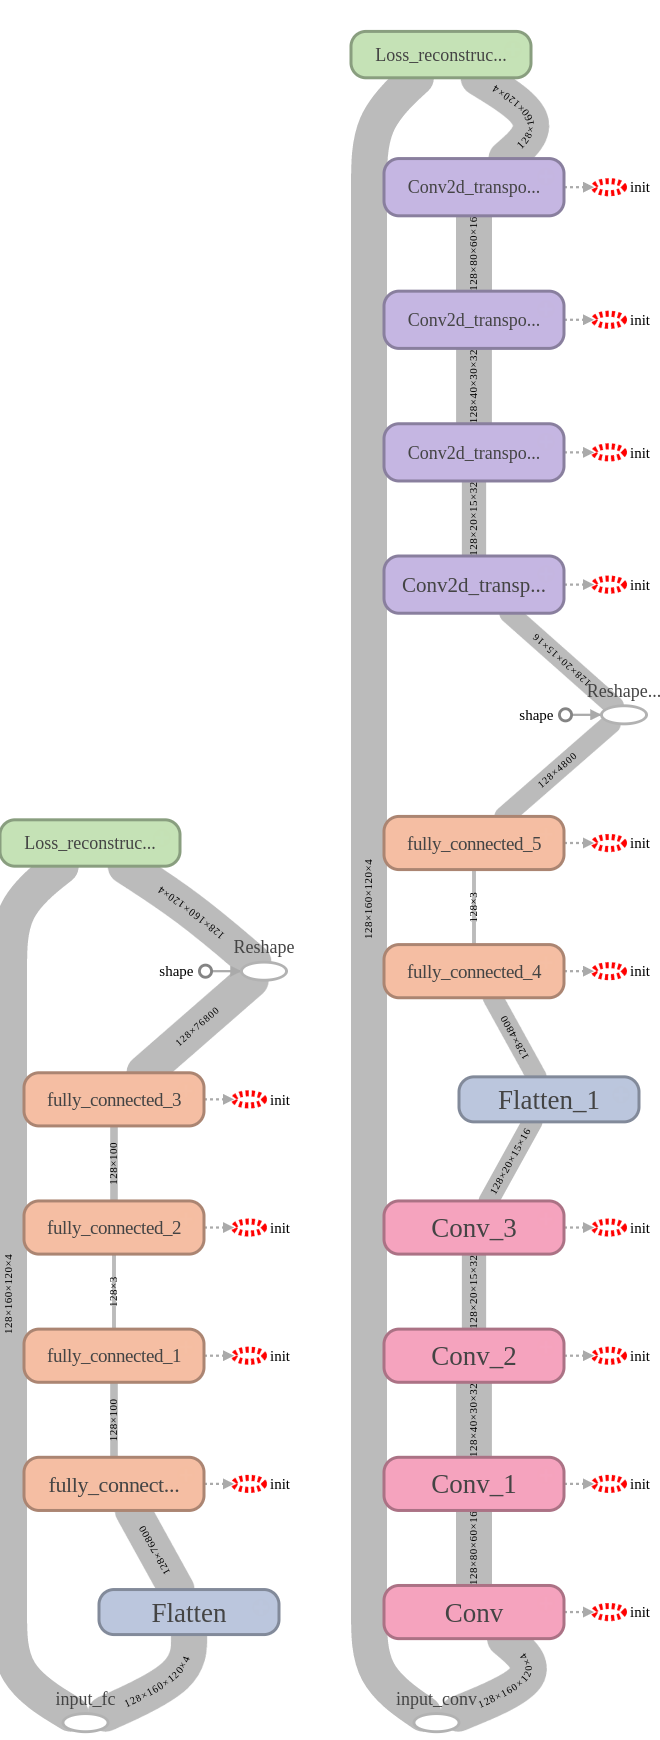
\includegraphics[width=\textwidth,height=\textheight,keepaspectratio]{backbone_1.png}
  \caption{Network graph structure of a fully-connected autoencoder (left) and a convolutional autoencoder (right).}
  \label{fig:tf_graph_1}
\end{figure}
% TODO: split into a, b images
\begin{figure}[H]
  \centering
    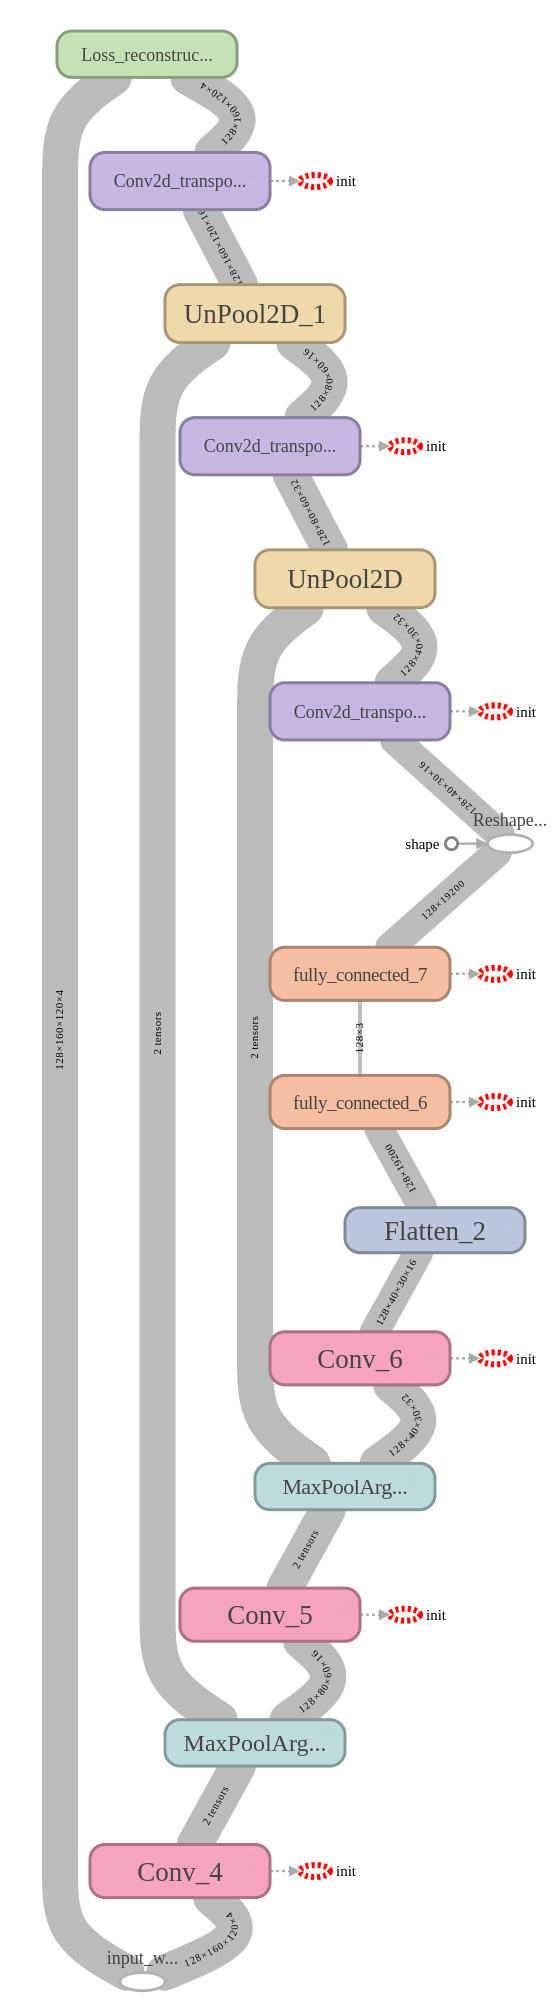
\includegraphics[width=\textwidth,height=\textheight,keepaspectratio]{backbone_2.png}
  \caption{Network graph of a What-Where Autoencoder with 3 pooling and unpooling layers.}
  \label{fig:tf_graph_2}
\end{figure}

\section{Model pre-training}

Xavier initialization provides good initial parameters to allow robust gradient backpropagation through a deep neural network architecture.
This approach provides alike learning rates across layers of the network.
It also decreases the chances of a neuron dying-out during initial training steps.
We can view Xavier initialization as a method, increasing chances of effectively using full network capacity during learning.

Yet, Xavier initialization does not guarantee, that a good local minima will be found.
Another robust approach to initialize network weights is reusing the weight of an already trained model.
This can be done by using layer weights, learned on a different dataset, or by using different objective function during initial phase of the training, as stacked autoencoders do \cite{Yosinski2014}.
We will refer to the later case as to \textit{model pre-training}.

We have next motivation for model pre-training.
In our early experiments we discovered high instability of the training process.
That is to say, an autoencoder based model learned to produce the same output image regardless of the input.
We assume, that this single output was a solution for minimization of average $L_{reco}$ on the complete training set.

We discovered that this instability can be explained by one of the next 2 factors:
\begin{enumerate}
  \item Extremely high compression rates. Trying to represent 76800 dimensional inputs in a 6- or lower-dimensional space is highly non trivial. Decreasing the compression rate always resulted in a more stable training.
  \item Noisy $L2$ loss. Neighboring pixels of a computer game images often have sharp differences and therefore are less correlated between each other.
  While we are trying to discover spatial structure using pixel-wise means squared error (MSE), such low correlation can be detrimental to the learning process.
  The reason is, that neighboring pixels can look as different from target value as remote pixels of the image.
  Which means that a small errors in the spatial transformations of the data can result in as high error as a large spatial transformations.
  These impedes learning process.
\end{enumerate}
% TODO: insert information about L2 error for neigboring pixels
% Mathieu2015 - MSE issues

From these two issues we can naturally deriver several methods for tackling this problem.
First, we can increase dimensionality of the encoding space, thus decreasing the compression ratio of the data.
Unfortunately, this would negatively effect the goal of this work: extracting low-dimensional interpretable features.
Therefore, we propose to improve the learning process by mitigating the noisy nature of the mean squared error.

We propose a model pre-training procedure that would incentivize learning of spatial information by the feature extractor (encoder).
We suggest, that increasing correlation of the neighboring pixels would result in at least local differentiability of spatial-dependent components of the latent feature space.
This quality should positively impact probability of learning latent representation of, specifically, spatial features by gradient descent.

In particular, we propose using training data to generate inputs for pre-training with higher local correlation between pixels.
We suggest using Gaussian blur as a preprocessing step to produce such data.
Next formula describes the transformation for each pixel of the image:

\begin{equation}
  G(x, y, \sigma) = \frac{1}{2\pi\sigma^2}\exp^{-\frac{x^2+y^2}{2\sigma^2}}
\end{equation}
where $(x, y)$ is relative position of the effected pixel to the source of transformation, $\sigma$ is real-valued parameter of the transformation.

Our pre-training technique is therefore dependent on two parameters: blur $\sigma$ and number of pre-training steps $N$.
We perform pre-training in scheduled way, by decreasing $\sigma$ linearly during the pre-training phase.
This allows smooth adaptation of the model parameters to the actual training data.

We can further argue that necessity of model pre-training can be explained by the real-world limitations of existing neural models.
Despite neural networks being universal approximator \cite{Debao1993}, some concepts might appear notoriously difficult to learn.
One recent example of such case is illustrated by learning identity mapping \cite{He2015}.
Authors prove, that even such trivial mappings as $f(x)=x$, while having positive effect on network performance, will not be learned as an intermediate mapping of a deep network.
We believe, that blurring the image is also one of the difficult concepts for neural networks.
In context of convolutional models, where de-facto standard is using $3 \times 3$ convolutions \cite{Szegedy2016a}, learning the effect of pixels being $N$ positions apart would require a convolutional architecture of depth at least $N/2$.

Altogether, we summarize our pre-training algorithm on listing \ref{alg:pretr}.

% !TEX root = ../thesis.tex

\begin{algorithm}[H]
 \KwData{X  \text{ (Train set)}}
 \KwResult{$\theta \text{ (Learned weights)}$}

 $\textbf{Require: } \sigma\text{: maximum blur distortion value}$

 $\textbf{Require: } N \text{: number of pre-training steps}$

 $\theta \gets \theta_0 \text{ (Xavier Initialization)}$

 \For{i in N}{

  $\sigma_i \gets (1 - \frac{i}{N})*\sigma \text{ (Calculate distortion parameter for current step)}$

  $X_i \gets \text{ Select minibatch examples i.i.d. from $X$}$

  $\hat{X_i} \gets \sigma(X_i, \sigma_i) \text{ (Apply distortion to the minibatch)}$

  $\theta \gets train\_minibatch(\theta, \hat{X_i}) \text{ (Perform a training step using distorted input)}$

 }

 \Return $\theta$

 \caption{Pre-training procedure for spatial-feature extraction}\label{alg:pretr}

\end{algorithm}

% TODO: finish the thought, add some math

\section{Manifold learning}\label{ss:mf}

While Variational Autoencoders and Generative moment matching networks can successfully learn dense data manifold, those models make no assumption about the nature of the manifold space \cite{Li2015, Ren2016, Kingma2013}.
In this section we describe our regularization techniques to incentivize manifold construction in more interpretable form.
For instance, we would like the manifold space to have local resemblance of the Euclidean space.
Also, we prefer to have predictable density of the data in the manifold space.

\subsection{Predictive objective}

With predictive objective we would like to explore the temporal relation of the data.
Training data is represented as one or multiple sequences of images.
Each sequence contains information about some unspecified arbitrary movement of an actor (player) through the environment (game).
This type of data contains at least two structural dependencies: correlation of information within each single image and temporal dependencies between frames.
While structural dependency within a single image is observed by the model at once for each input, temporal relation of the data is not taken into account.
With predictive objective we would like to create additional constrain on the model, that would allow learning of that temporal dependence of the data.

Let's first try to describe minimum necessary number of degrees of freedom.
Let's assume that the environment (a game map, or a building) is fixed, has no moving objects and does not change over time.
In that case we can construct the first person view of player given next inputs:
\begin{enumerate}
  \item $x, y, z$ - axes coordinates of the player within the environment,
  \item $\phi, \theta, \psi$ -  - roll, pitch, yaw angles depending on the orientation of player's view to coordinate axis,
  \item $\alpha$ - angle of players view.
\end{enumerate}

We can safely assume, that angle $\alpha$, as well as other possible output specific parameters, remains constant over the time.
In that case, we have in total 6 variables.
Namely, vectors of actor's view and position.
Lets assemble them into a players parameter vector $p=(x, y, z, \phi, \theta, \psi)$.
Note, that variables $x, y, z, \phi, \theta, \psi$ are independent from each other in the general case.
Lets also introduce a function $f(t)=p_t$, extracting player's positional information over time $t$.
From our empirical knowledge about players parameter vector $p_t$ we know, that $f(t)$ is a continuous function.

Let's assume, that encoder part of the network $e(x_t)= \hat{p_t}$, where $x_t$ is an image input at time $t$, successfully reconstructs the trajectory ${x_0, \ldots, x_N}$ on some manifold $M$.
Than we can state, that a local neighborhood of each point on the manifold $\hat{p_t}$ resembles continuous space of vector $p$, by the definition of a manifold.
Therefore, for any small neighborhood on the manifold we can approximately apply geometrical operations as in Euclidean space.

To add predictive objective we shall rely on the fact, that image at time $t_i$ is statistically dependent on whole sequence of previous images ${t_0, \ldots, t_{i-1}}$.
Given information ${t_0, \ldots, t_{i-1}}$ we can try to predict information about at time $i$.
While in the space of input images this task not trivial, in the space of player parameters $p$ we can simply approximate next position $p_{t+1}$ by current movement direction.
In other words, we can expect, that next transition of the player during small time period $\epsilon$ would be a lot like previous transition over the same period of time.
If we express it as $p_i = p_{i-1} + \delta_{i-1}$ we can expect that $\delta_i \approx \delta_{i-1}$ for sufficiently small time step. Deriving from that, we can construct next prediction procedure:
\begin{equation}
  \begin{aligned}
    &p_{i+1} = p_i + \delta_i \approx p_i + \delta_{i-1},\\
    &p_i + \delta_{i-1} = p_i + (p_i - p_{i-1}) = 2*p_i - p_{i-1}, \\
    &p_{i+1} \approx 2*p_i - p_{i-1}
  \end{aligned}
\end{equation}

At the same time, for sufficiently small values of $\delta$ we can expect this approximation to hold in the manifold space:
\begin{equation}
  \hat{p}_{i+1} \approx 2*\hat{p}_i - \hat{p}_{i-1}
\end{equation}

This procedure is schematically depicted on figure \ref{fig:m_pred}.

Unfortunately, the discretization of the video stream of the training data does not guarantee sufficiently small transitions between consecutive frames.
This is especially true for changes in the vie angle ($\phi, \theta, \psi$), since they can appear almost instantaneously and typically cause immense changes in terms of mean squared error.

\begin{figure}[h!]
  \centering
    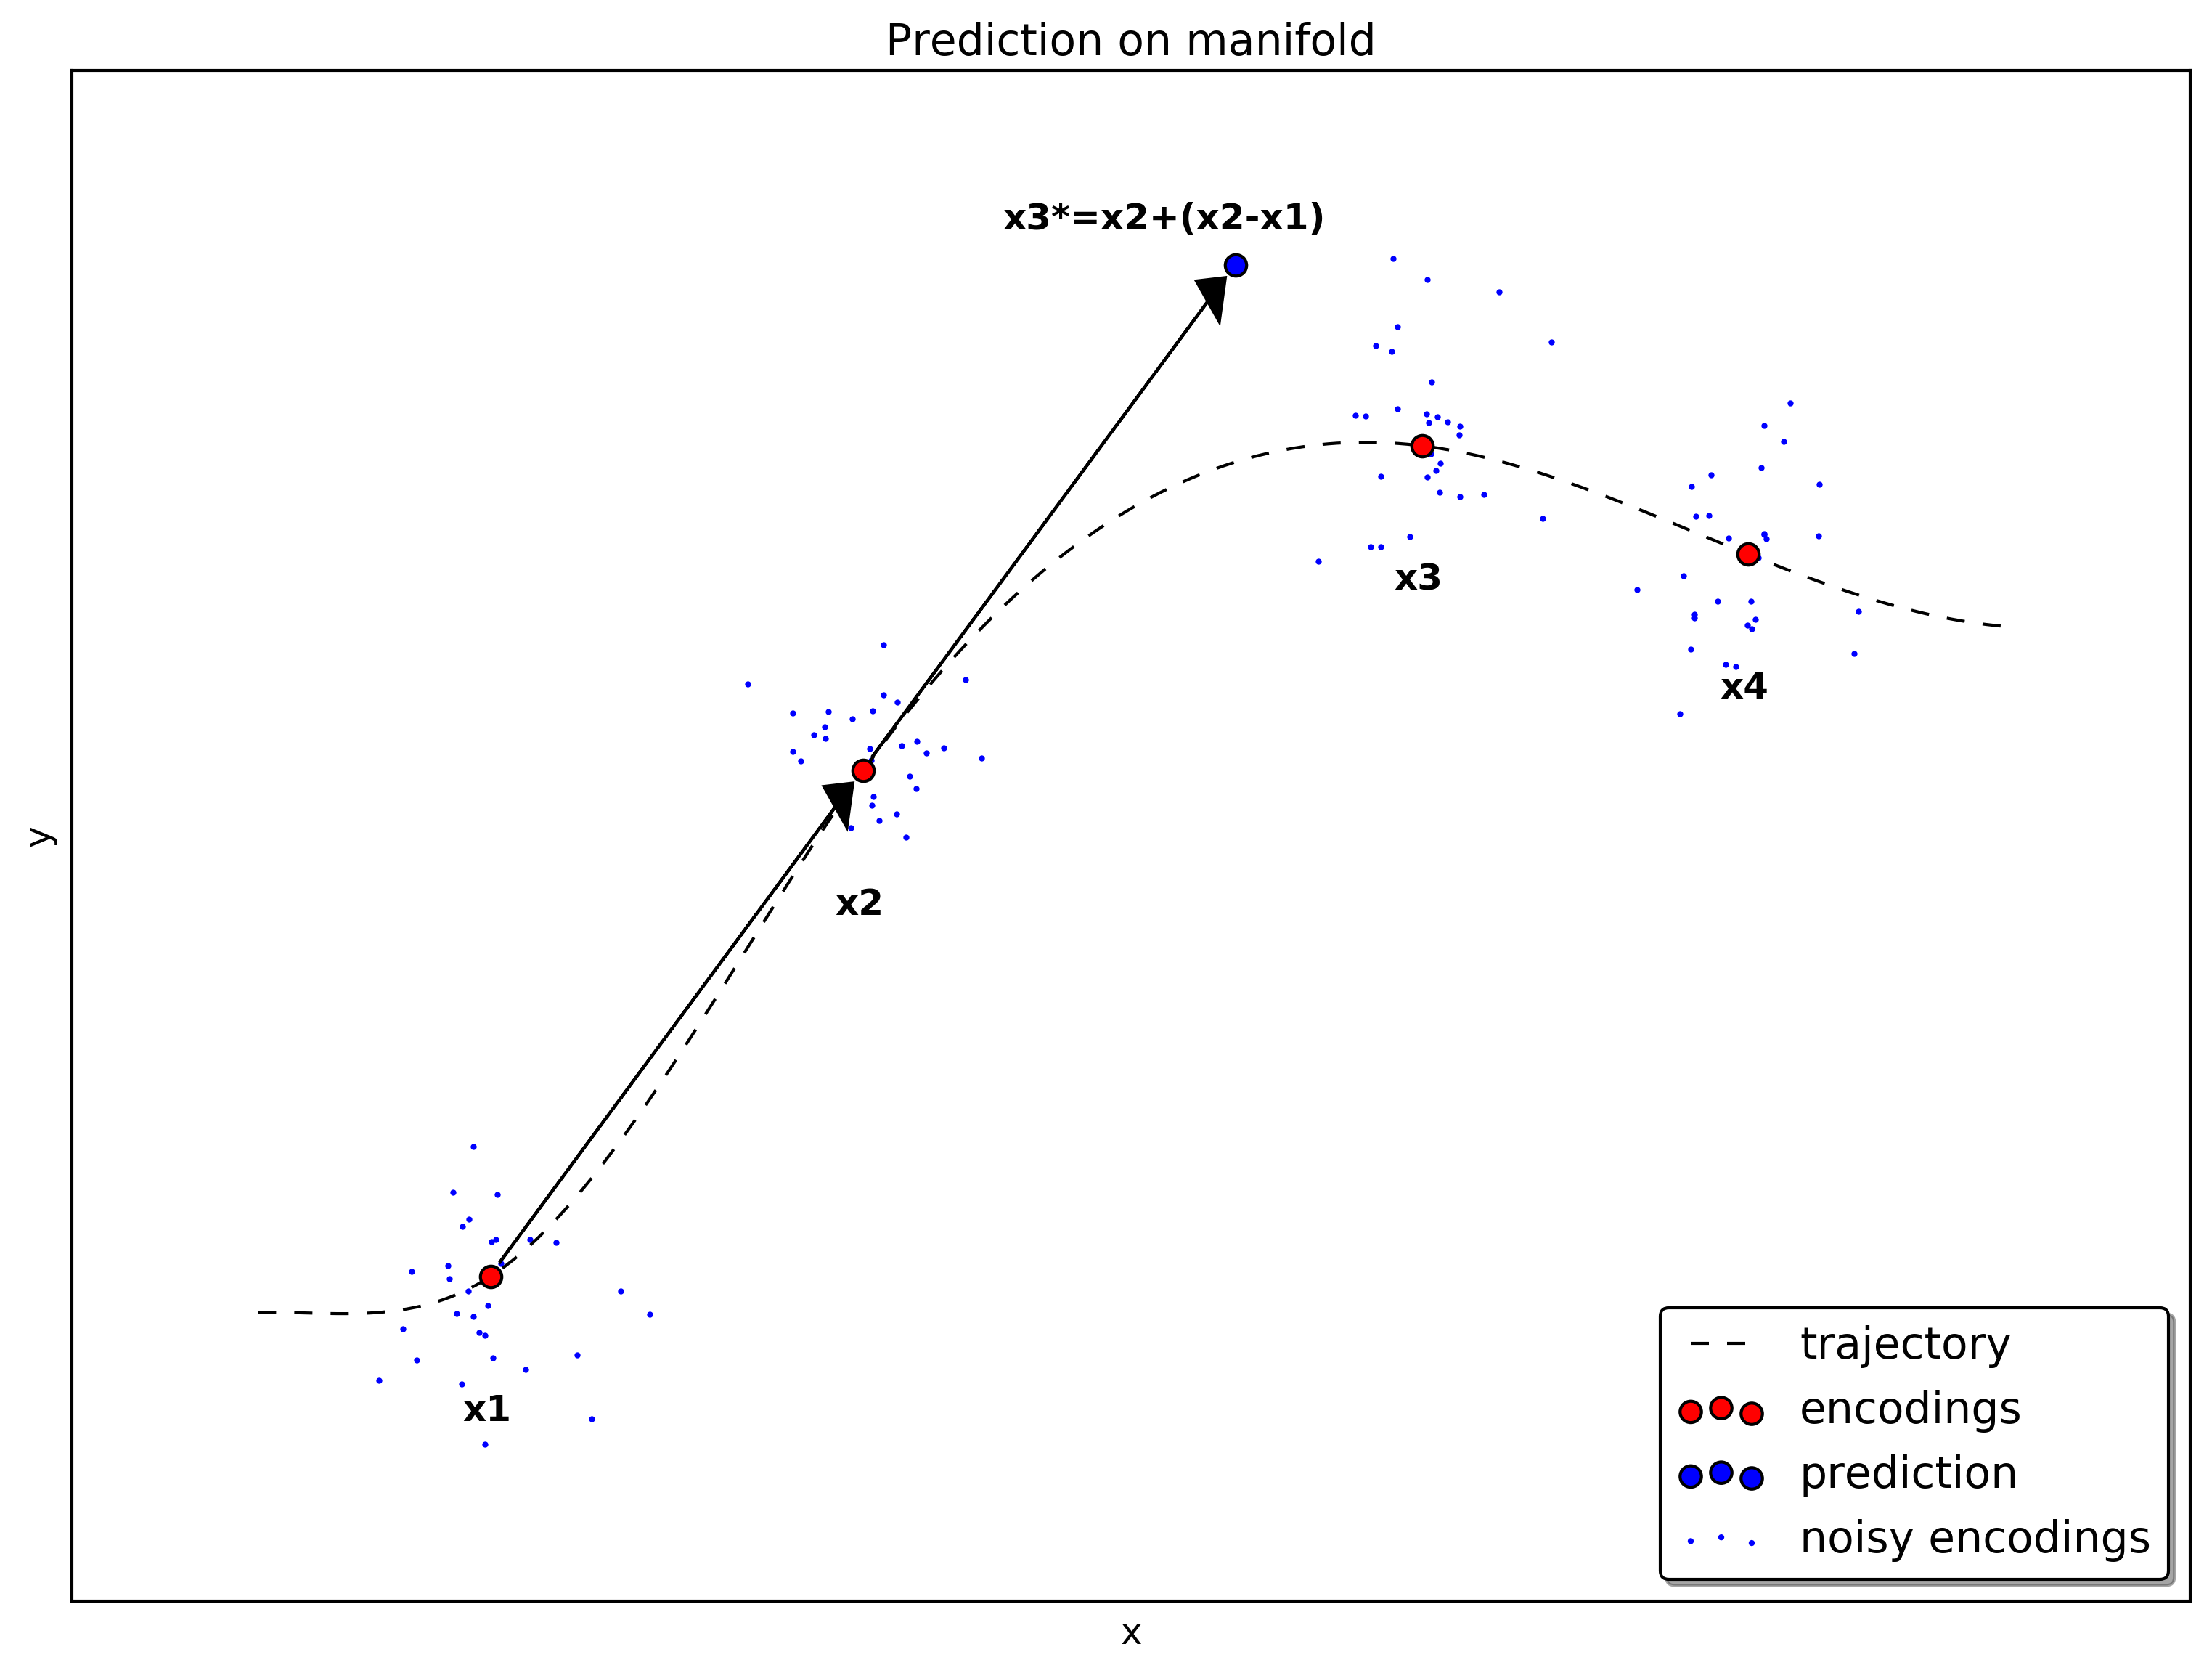
\includegraphics[width=0.85\textwidth,height=0.85\textheight, keepaspectratio]{prediction}
  \caption{Approximating position of encoding of frame $x_3$ by the encodings of two previous frames $x1, x2$ on the manifold trajectory.}.
  \label{fig:m_pred}
\end{figure}

% TODO: add a couple of words about model changes and reconstruction error

\subsection{Denoising regularization}

Early experiments showed largely uneven density of the manifold projection.
In particular cases this led to \textit{lumps} of images concentrated in a small region of the projection space.
From observation, images in the same lump tend to show high similarity between each other.

This behavior can be explained by largely uneven similarity between images across the training set.
For instance, let's says a single step along some trajectory is represented by $N$ discrete time-steps and, therefore, $N$ distinct sequential image inputs.
We can argue, that 2 distinct $N$-sequences from different parts of the trajectory might have highly different variation within the sequence.
As, for example, a single step towards the wall would cause either significant or almost unnoticeable change of the view depending on the distance from the wall.

High contrast of the degree of pair-wise image similarity across the dataset means, that alike errors in determining current position $p_i$ would cause highly uneven reconstruction error $L_{reco}$ depending on position $p_i$.
This, in turn, would lead to smaller gradient values during the learning process.
In the extreme case, gradients produced within regions of high similarity can be comparable or smaller than the noise of gradients of less similar regions.

To resolve this issue we propose using noise injection in the manifold space.
We suggest, that noisy embeddings would allow to enforce a minimum distance between input prototypes in the embedding space.
This minimum distance should allow to increase size of the regions around lumps, therefore gradually decreasing density in this regions.
As a result, we expect high density regions to become more robust against gradient noise, produced by less dense and more error-wise noisy inputs.

Injecting noise in the embedding space:
\begin{equation}
  x_i^* = x_i + \epsilon*G^n(0, 1)
\end{equation}

\subsection{Density regularization}

Despite continuous nature of actors movements, we have access only to discretized data in form of video frames.
This discretization sometimes results in sharp changes in the visual data in subsequent frames.
Low similarity in terms of reconstruction error of such frames leads to low similarity in the encoding space i.e. large gaps between consecutive frames.
Within such a region we can not longer argue about local resemblance of the manifold to a Euclidean space, continuous assumption about data at hand does not hold any longer.

Sharp changes in density of the manifold make it harder to argue about interpretability and quality of the learned concepts.
Furthermore, our experiments has shown, that manifolds with large number of low density regions tend to create larger number of self intersections, further complicating the interpretation of the learned features.

We, therefore propose a low-density regularization to account for regions with sharp changes.
We suggest using an additional error term during the training phase to penalize large distances between consecutive frames, therefore dragging them closer together.
Such regularization would compete with the reconstruction objective of the autoencoder network.
But our main interest is interpretable feature extraction, not archiving perfect reconstruction of the images.

Therefore, we calculate euclidean distance between pair of subsequent images:
\begin{equation*}
d(x_t, x_{t+1}) = \Big(\sum^i { (x_{t,i}-x_{t+1, i})^2}\Big)^{\frac{1}{2}}
\end{equation*}
And penalize distances exceeding certain constant value $d_{max}$:

\begin{equation*}
  L_{dens} = \gamma*\max(0, d(x_t, x_{t+1})-d_{max})
\end{equation*}
where $\gamma$ is a constant parameter defining contribution of the density regularization in total loss.


Figure \ref{fig:model} summarizes our modification to the autoencoder architecture on a single schema.

% !TEX root = ../thesis.tex

\begin{figure}

\centering
\begin{tikzpicture}
%   [align=center,node distance=2cm]
  [
    every label/.style={align=center},
  	lbl/.style={draw, circle, minimum width=0mm, minimum height=0mm, inner sep=0pt},
    vlbl/.style={draw, circle, minimum width=0mm, minimum height=0mm, inner sep=0pt},
    state/.style={draw, circle, minimum width=6mm, minimum height=6mm, inner sep=3pt},
    param/.style={draw, rectangle, minimum width=6mm, minimum height=6mm, inner sep=3pt},
    func/.style={draw, rectangle, minimum width=2.9cm, minimum height=1cm, inner sep=3pt, rounded corners},
    relu/.style={draw, rectangle, minimum width=1cm, minimum height=1cm, inner sep=3pt, rounded corners},
    enc/.style={draw, trapezium, shape border rotate=-180, minimum width=0.7cm, minimum height=0.7cm, inner sep=2pt},
    dec/.style={draw, trapezium, shape border rotate=90,  minimum width=0.7cm, minimum height=0.7cm, inner sep=2pt},
    loss/.style={draw, diamond, minimum width=1cm, minimum height=1cm, inner sep=2pt},
    node distance=20mm,
    classical/.style={dashed,->,shorten >=4pt,shorten <=4pt,>=stealth},
    % Define arrow style
    pil/.style={
           ->,
           thick,
           shorten <=2pt,
           shorten >=2pt,}
%     dotted/.style={dotted,-,shorten >=4pt,shorten <=4pt,>=stealth}
  ]
%   \node (x) [state, label=left:$X_1$] {$x_1$};
  \node (x1) [state, label=left:$X_1$] {$x_1$};
  \node (x2) [state, below of=x1,label=left:$X_2$] {$x_2$};
  \node (enc1) [enc, right=.5cm of x1] {$E$};
  \node (enc2) [enc, right=.5cm of x2] {$E$};
  \node (e1) [state, right of=enc1,shift={(-0.5,0)}] {$e_1$};
  \node (e2) [state, right of=enc2,shift={(-0.5,0)}] {$e_2$};

%   prediction
  \node (pred) [func, right=1.0cm of e2,label=below:Prediction] {$(2*e_2-e_1)$};
  \node (e3) [state, right=.5cm of pred,label=below:prediction] {$e_3^*$};

%   noise
  \node (noise) [func, below right=1.2cm and 1.13cm of e2, label=below:Inject noise] {$e_2 + \epsilon*N^d(0, 1)$};
  \node (n2) [state, right=.5cm of noise,label=below:noisy] {$n_2$};
  \node (eps) [param, left=1.cm of noise] {$\epsilon$};

%   distance
  \node (dist) [func, below=1cm of noise,label=below:Distance] { $\text{  }|e_1, e_2|_2^2-d_{max}\text{  }$ };
%   \node (d) [state, right=.5cm of dist,label=below:distance] {$\delta d$};
  \node (rel) [relu, right=0.5cm of dist,label=below:ReLU] {$max(0,\delta d )$};
  \node (dmin) [param, left=1.cm of dist] {$d_{m}$};

%   decoding
  \node (decp) [dec, right=.5cm of e3] {$D$};
  \node (dec2) [dec, above of=decp] {$D$};
  \node (decn) [dec, right=.5cm of n2] {$D$};

  \node(l2)[loss, right=.5cm of dec2, label={[xshift=0.8cm]below:{Autoencoder objective}}]{$L_{x1}$};
  \node(lp)[loss, right=.5cm of decp, label={[xshift=0.9cm]below:{Predictive regularization}}]{$L_{x3}$};
  \node(ln)[loss, right=.5cm of decn, label={[xshift=0.9cm]below:{Denoising regularization}}]{$L_{x2}$};
  \node(ld)[loss, below of=ln, label={[xshift=0.9cm]below:{Density regularization}}]{$L2$};


%   \node (le3) [state, right of=lp] {$x_3$};
%   \node (le2_1) [state, right of=l2] {$x_2$};
%   \node (le2_2) [state, right of=ln] {$x_2$};

  \node (a) [param, right=.9cm of lp] {$\alpha$};
  \node (b) [param, right=.9cm of ln] {$\beta$};
  \node (g) [param, right=.9cm of ld] {$\gamma$};

%   labels
  \node (lbl2) [lbl, above of=enc1, yshift=-1cm, label=above:\large{Encoder}]{};
%   \node (lbl3) [lbl, left of=lbl2,label=above:\large{Inputs}]{};
  \node (lbl5) [lbl, above of=l2, yshift=-1cm, label=above:\large{Losses}]{};
  \node (lbl4) [lbl, above of=dec2, yshift=-1cm, xshift=-0.3cm, label=above:\large{Decoder}]{};
  \node (lblx) [lbl, left of=lbl4]{};
  \node (lbl1) [lbl,left of=lblx, xshift=0.7cm,label=above:\large{Calculations}]{};
%   \node (lbl6) [lbl, right of=lbl5, label=above:\large{Parameters}]{};

%   \node (vlbl_p) [vlbl, right of=a, label={[xshift=.5cm]left:\rotatebox{-90}{\large{Predictive}}}]{};
%   \node (vlbl_ae) [vlbl, above of=vlbl_p, label={[xshift=-.5cm]left:\rotatebox{-90}{\large{Autoencoder}}}]{};
%   \node (vlbl_n) [vlbl, below of=vlbl_p,label={[xshift=-0.5cm, align=center]left:{\rotatebox{-90}{\large{Denoising}}}}]{};
%   \node (vlbl_d) [vlbl, below of=vlbl_n, label={[xshift=.5cm]left:\rotatebox{-90}{\large{Density}}}]{};


%   arrows
%   \draw[->] (description) .. controls ([xshift=-4cm] description) and ([xshift=4cm] text) .. (text);
  \draw[->] (e2) .. controls ([xshift=1cm, yshift=-2cm] e2) and ([xshift=-.5cm] dist.north west) .. (dist);
  \draw[->] (e2) .. controls ([xshift=1cm, yshift=-1cm] e2) and ([xshift=-1cm] noise.north west) .. (noise);

  \draw[->] (e1) .. controls ([xshift=1cm] e1.east) and ([xshift=-.5cm] pred.north west) .. (pred);
  \draw[->] (e1) .. controls ([xshift=-1cm, yshift=-2cm] e1) and ([xshift=-2.0cm] dist.west) .. (dist);


  \draw[->] (x2) -- (enc2);
  \draw[->] (enc2) -- (e2);
  \draw[->] (e2) -- (pred);
  \draw[->] (pred) -- (e3);
  \draw[->] (e3) -- (decp);
  \draw[->] (decp) -- (lp);
%   \draw[->] (le3) -- (lp);
	\draw[->] (a) -- (lp);

  \draw[->] (x1) -- (enc1);
  \draw[->] (enc1) -- (e1);
  \draw[->] (e1) -- (dec2);
  \draw[->] (dec2) -- (l2);
%   \draw[->] (le2_1) -- (l2);
	\draw[->] (b) -- (ln);

%   \draw[->] (dist) -- (d);
%   \draw[->] (d) -- (rel);
  \draw[->] (dist) -- (rel);
  \draw[->] (rel) -- (ld);

  \draw[->] (noise) -- (n2);
  \draw[->] (n2) -- (decn);
  \draw[->] (decn) -- (ln);
%   \draw[->] (le2_2) -- (ln);
  \draw[->] (g) -- (ld);

  \draw[->] (eps) -- (noise);
  \draw[->] (dmin) .. controls ([xshift=-.2cm] dist.south west) .. (dist);



%   	\draw [color=gray,thick](-1.5,-1) rectangle (15.5,1.5);
% 	\node at (-0.5,1) [above=5mm, right=0mm] {\textsc{first-order noise shaper}};
% 	\draw [color=gray,thick](-0.5,-9) rectangle (12.5,-5);
% 	\node at (-0.5,-9) [below=5mm, right=0mm] {\textsc{second-order noise shaper}};

%   \coordinate (aux) at (x1.south) -- (x1.south|-x2.north);
%   \draw[dashed]([xshift=-1cm]x1.north west|-aux) -- ([xshift=1cm]x2.north east|-aux);


%   \draw (0,-1) -- (4,-1);
\end{tikzpicture}
\caption{Spacial feature extractor with regularization terms.}
\label{fig:model}
\end{figure}

